\subsection{Azize Euphemia Kilisesi}
\indent\indent Azize Euphemia, MS 307 yılında Ares için düzenlenen şenliklere katılmayı reddettiği için Khalkedon'da(bugün Kadıköy) tutuklanmıştır. Ölüm tarihini ise kaynaklar 16 Eylül 307 olarak bildirmektedir. Daha sonra Hıristiyanlıkta şehit olarak kabul edilecek Euhemia'nın bedeni bütün olarak bir tabutun içinde muhafaza edildi. Tam olarak ne zaman yapıldığı bilimese de 4.yüzyılın sonlarına doğru Khalkedon'da, Euphemia adına yapılmış bir kilisenin varlığı bilinmektedir. 451 yılında Khalkedon konsili, bu kilisede toplanmıştır. 7.yüzyılın başındaki Pers akınları ile hasar gören kiliseden Euphemia'nın \textit{bozulmamış bedeni} buradan alınıp, Konstantinopolis surları içine getirilmiştir. Daha sonra Hippodrom'un bitişiğindeki Antiokhos sarayının yanına Euphemia adına yeni bir kilise inşa edildi. Bu kilise, Hippodrom'daki Azize Euhemia Kilisesi olarak anılmıştır.\cite{euphemia}\newline
\indent 1951-52 yıllarında, Adalet Sarayı'nın yapımı için ifa edilen kazılarda ortaya çıkan kiliseden günümüze sadece silüeti kalmıştır. Yerdeki kalıntılarda bir apsis göze çarpıyor. Apsisin karşısında kalan ve tahminen girişin yer aldığı duvar kısmen ayaktadır. Bu duvar üzerindeki freskolar da yine kısmen görülebilmektedir.
\begin{figure}[H]
    \centering
    \subfigure[Fresko - 1]{
        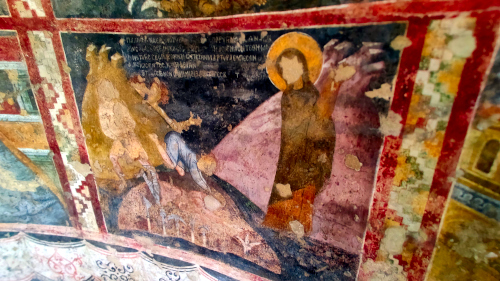
\includegraphics[height=0.15\textheight]{assets/euphemia_fresco_1.jpg}
    }
    \subfigure[Fresko - 2]{
        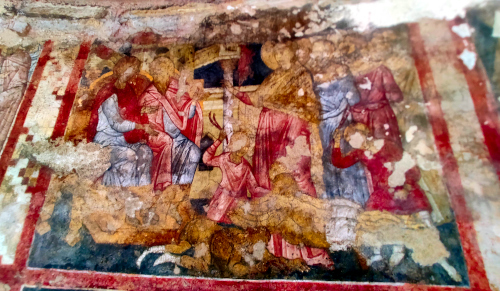
\includegraphics[height=0.15\textheight]{assets/euphemia_fresco_2.jpg}
    }
    \subfigure[Duvar]{
        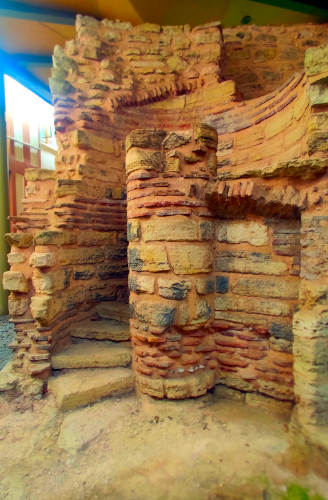
\includegraphics[height=0.15\textheight]{assets/euphemia_wall.jpg}
    }
    \subfigure[Apsis]{
        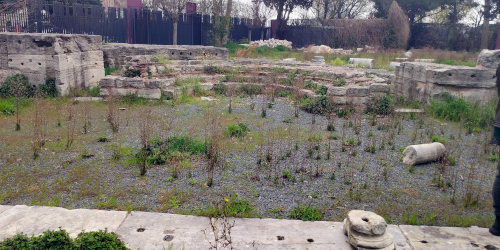
\includegraphics[height=0.2\textheight]{assets/euphemia_apsis.jpg}
    }
    \caption{Azize Euphemia Kilisesi Kalıntıları}
\end{figure}